\section{Theoretical Foundations: Two-Qubit $CZ$ gate}

This section establishes the theoretical framework and physical architecture necessary for understanding and
implementing the two-qubit CZ gate. We examine the operational principles of the adiabatic CZ gate and discuss why the
Slepian pulse shape has traditionally been favored for control pulses.
% In this section, we establish the theoretical framework and physical architecture necessary for understanding and
% implementing the two-qubit $CZ$ gate.
% We see how the adiabatic $CZ$ gate operates and why Slepian pulse shape has long been used for the control pulse.
We use some symbols for different purposes in the $X$ and $CZ$ gates. When confusion arises, consult the notation table
in \tref{tab:notation} located immediately following the abstract.
\subsection{SQUID loop and $Z$-control}
\begin{figure}[bthp]
  \centering
  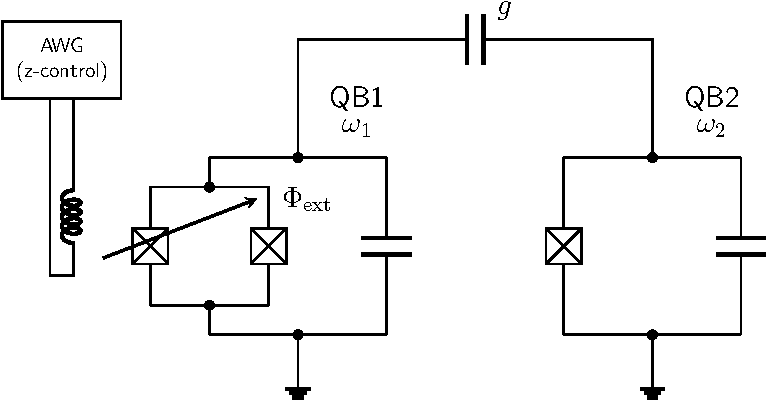
\includegraphics[width=0.8\textwidth]{fig/fig_z-ctrl.pdf}
  \caption{Target qubit architecture in our work. A tunable-frequency QB1 and a fixed-frequency QB2 are capacitively
    coupled with factor $g$.}
  \label{fig:z-ctrl}
\end{figure}
In superconducting quantum architectures, the ability to dynamically tune the transition frequency of a qubit is
essential for realizing the adiabatic $CZ$ gate.
This tunability is achieved by replacing the single Josephson junction of a standard
transmon with a superconducting quantum interference device (SQUID) loop as depicted in \fref{fig:z-ctrl},
which is then threaded by a localized magnetic
flux $\Phi_\text{ext}$ controlled via a dedicated microwave transmission line known as the $Z$-control line (or flux line).
% In \fref{fig:z-ctrl},
% \begin{equation}
%   % \begin{align}
%   \omega_1(\Phi_{\text{ext}})   = \frac{1}{\hbar} \left( \sqrt{8E_JE_C} \sqrt[4]{d^2 + (1 - d^2)
%       \cos^2(\pi \frac{\Phi_{\text{ext}}}{\Phi_0})} - E_C \right),
%   % \end{align}
%   \label{eq:flux}

\subsection{Qubit Architecture}
The system we consider is illustred in \fref{fig:z-ctrl}.
It is a system of two capacitively coupled transmon qubits, one fixed-frequency (QB2) and the other frequency tunable (QB1).
The simplified dispersive Jaynes-Cummings Hamiltonian for this system can be modeled as:
$$H = \sum_{i=1,2} \left( \omega_i \hat{a}_i^\dagger \hat{a}_i + \frac{\alpha_i}{2} \hat{a}_i^\dagger \hat{a}_i^\dagger \hat{a}_i \hat{a}_i \right) + g(\hat{a}_1^\dagger + \hat{a}_1)(\hat{a}_2^\dagger + \hat{a}_2) ,$$
where $g$ denotes the capacitive coupling strength between the two qubits, $\hat{a}_i^\dagger$ and $\hat{a}_i$ represent the
creation and annihilation operators for qubit $i$, respectively, and $\alpha_i$ defines the anharmonicity of qubit $i$.
Note that we use $\alpha$ for anharmonicity in discusion of the $CZ$ gates.
We use $\Delta$ and $\omega_i$ to denote different things. ($\Delta$ instead denotes the effective coupling strength
$2\sqrt{2}g$)
\subsection{Adiabatic Implementation}
CZ gate is a two-qubit gate that applies a phase flip to the target qubit if the control qubit resides in the state
$\ket{1}$. In the computational basis $\{\vert{}00\rangle, \vert{}01\rangle, \vert{}10\rangle, \vert{}11\rangle\}$, the
ideal unitary evolution is represented by a diagonal matrix:
\begin{equation}
  U_{\mathrm{CZ}}=\begin{pmatrix}
    1 & 0 & 0 & 0  \\
    0 & 1 & 0 & 0  \\
    0 & 0 & 1 & 0  \\
    0 & 0 & 0 & -1
  \end{pmatrix}.
\end{equation}
% The adiabatic CZ gate is realized as syncing the QB1's frequency to QB2's, thereby creating an avoided crossing.
% By doing so, the energy of $\ket{11}$ and $\ket{20}$ become comparable.
To implement this gate, the frequency of QB1 is swept along a
prescribed trajectory $\omega_1(t)$ toward the avoided crossing, held or continuously varied for a duration $\tau_d$,
and then returned to its idle parking frequency.
In this process, $\ket{11}$ obtains/loses more phases than the other computational states, due to its stronger coupling
to $\ket{02}$.

By following Refs.~\cite{Ding2025,Martinis2014}, we review the theory behind the adiabatic implementaion of the $CZ$ gate and
the derivation of the leakage formula \eref{eq:leakage}.
\begin{theorem}[Adiabatic Theorem]
  If a quantum system is initially prepared in a non-degenerate energy eigenstate of a time-dependent Hamiltonian, and
  if that Hamiltonian is varied sufficiently slowly, the system will evolve continuously to remain in the corresponding
  instantaneous eigenstate of the evolving Hamiltonian up to an accumulated phase factor, given that there is a gap
  between the eigenvalue and the rest of the Hamiltonian's spectrum.
\end{theorem}
Consider a two level system with the following Hamiltonian
$$
  H(t)=\eps(t)\sigma_z + \Delta\sigma_x.
$$
According to the adiabatic theorem, if we prepare the state $\ket{0}$ and slowly vary the Hamiltonian and then retrace the
change back, the resulting state is $\ket{0}$ with phase accumulation.
The instantaneous eigenstates are
\begin{equation}
  \vert{}\psi_-\rangle = \begin{bmatrix} -\sin(\theta(t)/2) \\ \cos(\theta(t)/2) \end{bmatrix} \quad \text{and} \quad \vert{}\psi_+\rangle = \begin{bmatrix} \cos(\theta(t)/2) \\ \sin(\theta(t)/2) \end{bmatrix},
\end{equation}
with eigenenergies
\begin{equation}
  E_- = -\frac{1}{2}\sqrt{\varepsilon(t)^2 + \Delta^2} \quad \text{and} \quad E_+ = \frac{1}{2}\sqrt{\varepsilon(t)^2 + \Delta^2},
\end{equation}
where
\begin{equation}
  \theta(t) = \arctan\frac{\Delta}{\eps(t)}.
  \label{eq:theta}
\end{equation}
We denote the energy difference of these two instantaneous eigenstates as
\begin{equation}
  \omega(t) = \sqrt{\varepsilon(t)^2 + \Delta^2}.
  \label{eq:omega}
\end{equation}

\subsubsection{Calculation of Leakage Error} \label{subsec:leakage}
Consider a state
$$
  \ket{\psi} = \alpha \ket{\psi_{-}}+\beta\ket{\psi_+} = \alpha_0\ket{0}+\beta_0\ket{1}
$$
with rotational change of coefficients
\begin{align*}
  \alpha & = \alpha_0\cos\dfrac{\theta}{2} + \beta_0\sin\dfrac{\theta}{2},  \\
  \beta  & =  \beta_0\cos\dfrac{\theta}{2} - \alpha_0\sin\dfrac{\theta}{2}.
\end{align*}
Differentiating with respect to time, we obtain
\begin{align*}
  \dot{\alpha} & = \dfrac{-i\omega \alpha+\beta \dot{\theta}}{2}, \\
  \dot{\beta}  & = \dfrac{i\omega \beta-\alpha \dot{\theta}}{2}.  \\
\end{align*}
By expressing the coefficients in terms of the angles $\alpha = \cos (\Theta/2)$ and $\beta=e^{i\phi}\sin(\Theta/2)$, we can
define
$$
  \alpha^* \beta = \dfrac{\sin\Theta e^{i\phi}}{2}.
$$
Calculating the time derivative of this quantity yields
$$
  \frac{d}{dt}(\sin\Theta e^{i\phi}) = i\omega \sin\Theta e^{i\phi}  \pm  \dot{\theta}\cos\Theta.
$$
Plugging $\phi=\phi_{\text{initial}} + \int_0^t\,\omega(t^\prime)\,\dd t^\prime$ and
symplifying the expression gives the approximate leakage probability $P_e=|\sin(\Theta(T)/2)|^2$,
\begin{equation}
  % \frac{d}{dt}(\sin\Theta e^{i\phi}) = i\omega \sin\Theta e^{i\phi}  \pm  \dot{\theta}\cos\Theta
  P_e \approx \dfrac{1}{4}\, \left\lvert\, \int_0^T \,\dfrac{\dd\theta}{\dd t} e^{-i\int\omega(t^\prime)\,\dd t^\prime}\right\rvert^2,
  \label{eq:leakage}
\end{equation}
with $T$ being a gate duration.
% If we assume that the time derivative of $\ket{\psi_-}$ and $\ket{\psi_+}$ are small enough, $\ket{\psi}$ evolves accordingly to \begin{align*}
%   \dot{\alpha} & = -iE_- \alpha, \\
%   \dot{\beta}  & = -iE_+\beta,
% \end{align*}
% in other words,
% \begin{align*}
%   \dot{\alpha} & = \dot{\alpha_0}\cos\dfrac{\theta}{2} + \dot{\beta_0}\sin\dfrac{\theta}{2},  \\
%   \dot{\beta}  & =  \dot{\beta_0}\cos\dfrac{\theta}{2} - \dot{\alpha_0}\sin\dfrac{\theta}{2},
% \end{align*}


\subsubsection{Dynamical and Conditional Phase Accumulation}
% According to the adiabatic theorem, if the sweep rate is sufficiently slow compared to the energy gap at the avoided crossing,
% the system will remain in its instantaneous eigenstate. The dynamic frequency excursion imparts a continuous deformation
% on the $\vert{}11\rangle$ state, causing it to hybridize temporarily with $\vert{}02\rangle$ and acquire a dynamical phase.
% The total accumulated phase $\Phi_{11}$ on the $\vert{}11\rangle$ state is the time integral of its instantaneous eigenenergy
% $E_{11}(t)$:$$\Phi_{11} = -\frac{1}{\hbar} \int_{0}^{\tau} E_{11}(t) dt$$
% Alongside the avoided crossing, the other states than $\ket{11}$ also acquire dynamical phases.
% To find the net phase $\ket{11}$ accumulates, we need to subtract these phases.
% % Simultaneously, single-qubit dynamical phases $\Phi_{01}$ and $\Phi_{10}$ are acquired.
% The conditional phase $\phi_{\text{cond}}$ accumulated over the gate duration is calculated
% by isolating the two-qubit interaction phase from the single-qubit contributions:
% $$\phi_{\text{cond}} = \Phi_{11} - \Phi_{01} - \Phi_{10} + \Phi_{00}$$
% The gate is successful when the pulse amplitude and duration are calibrated such
% that $\phi_{\text{cond}} = \pi \pmod{2\pi}$.
During the sweep towards the avoided crossing, computational states other than $\vert{}11\rangle$ also accumulate
dynamical phases. To determine the net phase acquired by the $\vert{}11\rangle$ state, these single-qubit contributions
must be subtracted. Specifically, the conditional phase $\phi_{\text{cond}}$ accumulated over the gate duration is
calculated by isolating the two-qubit interaction phase from the single-qubit contributions,
$$\phi_{\text{cond}} = \Phi_{11} - \Phi_{01} - \Phi_{10} + \Phi_{00},$$
where $\Phi_{ij}$ denotes phase accumulation for the state $\ket{ij}$.
A successful gate operation requires calibrating the pulse amplitude and
duration such that $\phi_{\text{cond}} = \pi \pmod{2\pi}$.

\subsubsection{Nonlinear time transformation}
By applying a time transformation, we can simplify the leakage formula \eref{eq:leakage}.
Let the time variable of this new frame be $\tau$. Set
$$
  \Delta \dd \tau = \omega(t) \dd t,
$$
then
\begin{equation}
  \dd t = \dfrac{\Delta}{\omega(t)}\dd \tau = \sin \theta(t) \dd \tau.
  \label{eq:nonlinear_time_transform_differential}
\end{equation}
In integral form,
\begin{equation}
  t(\tau) = \int_0^\tau\,\sin\tilde{\theta}(\tau^\prime)\,\dd\tau^\prime.
  \label{eq:nonliniear_time_transform}
\end{equation}
The virtue of this transformation is clear if we plug \eref{eq:nonlinear_time_transform_differential} into \eref{eq:leakage},
\begin{equation}
  P_e = \dfrac{1}{4}\, \left\lvert\, \int_0^\tau\,\dfrac{\dd\tilde{\theta}}{\dd\tau}\, e^{-i\Delta \tau}\,\dd \tau \right\rvert^2.
  \label{eq:leakage_tau}
\end{equation}
The leakage error is expressed as the Fourier transform of $\dfrac{\dd\tilde{\theta}}{\dd \tau}$
at $\Delta$.


\subsection{Slepian pulses}

% In the context of pulse waveform optimization, the Slepian pulses, frequently referred to as discrete prolate spheroidal
% sequences (DPSSs), represent a family of orthogonal pulses specifically formulated to solve the problem of maximal
% energy concentration in both the time and frequency domains. Because Heisenberg's uncertainty principle dictates that a
% pulse cannot be strictly bounded in both time and frequency simultaneously, Slepian, Landau, and Pollack developed these
% sequences to answer a fundamental optimization question: how to optimally concentrate energy in one domain when the
% pulse is strictly confined in the opposing domain.

A (discrete) Slepian pulse is a finite-length discrete time signal which maximazes the energy concentration in a prescribed
frequency band $[-W,W]$.
The exact formula for this pulse can be derive by considering the following eigenvalue problem.

Consider a discrete-time pulse of finite length, denoted as $x[n]$ for $n = 0, 1, \dots, N-1$.
Its energy concentration in $[-W,W]$ is
\begin{equation}
  \frac{\int_{-W}^{W} \vert{}X(e^{i\omega})\vert{}^2 d\omega}{\int_{-\pi}^{\pi} \vert{}X(e^{i\omega})\vert{}^2
    d\omega},
  \label{eq:energy_concentration}
\end{equation}
where $X$ denotes discrete Fourier transform,
$$X(e^{i\omega}) = \sum_{n=0}^{N-1} x[n]e^{-i\omega n}.$$
The \eref{eq:energy_concentration} can be rewritten as
$$\dfrac{x^TAx}{x^Tx}$$
where $x$ is the vector form of the signal $x[n]$ and $A$ is a matrix with $A_{n,m} = \frac{\sin 2\pi W(n - m)}{\pi(n - m)}$.

$A$ has $N$ eigenvalue solutions and the eigenvector corresponding to the second largest eigenvalue satisfies
anti-symmetric property $x[n] = -x[N-1-n]$.

\subsection{Limitations of Slepian Pulses}
While the Slepian pulse is widely utilized and exhibits an excellent spectral profile with exceptionally low sidelobes,
it is not strictly optimal for this specific application.
As demonstrated in \eref{eq:leakage_tau}, the leakage error depends exclusively on the Fourier transform evaluated at the precise
frequency $\Delta$. Consequently, this leaves significant room for further targeted waveform optimization.
